\documentclass[aspectratio=169, table]{beamer}

\usepackage[utf8]{inputenc}
\usepackage{listings} 

\usetheme{Pradita}

\subtitle{MTI104 - IT Services}

\title{Session-03:\\\LARGE{IHolistic Approach to Service \\Management: Four Dimensions}}
\date[Serial]{\scriptsize {PRU/SPMI/FR-BM-18/0222}}
\author[Pradita]{\small{\textbf{Alfa Yohannis}}}

\begin{document}

\frame{\titlepage}

\begin{frame}
	\frametitle{Service Management Overview}
	\begin{itemize}
		\item Service management is not linear.
		\item Multiple aspects and components create a service.
		\item Both creation and consumption sides must collaborate.
		\item Components must align to create value.
		\item These components are organized into four dimensions.
		\item This chapter explores these dimensions.
		\item External factors also influence service delivery and consumption.
	\end{itemize}
\end{frame}

\begin{frame}
	\frametitle{The Four Dimensions of Service Management}
	\begin{itemize}
		\item Balance is essential in service management.
		\item Services require all constituent components for growth.
		\item Four key dimensions identified:
		\begin{itemize}
			\item Organization and people
			\item Information and technology
			\item Suppliers and partners
			\item Value streams and processes
		\end{itemize}
		\item These dimensions must work in unison.
		\item IT services operate in rapidly changing environments.
	\end{itemize}
\end{frame}

\begin{frame}{Four dimensions of service management}
	 \frametitle{ Four dimensions of service management}
\begin{center}
	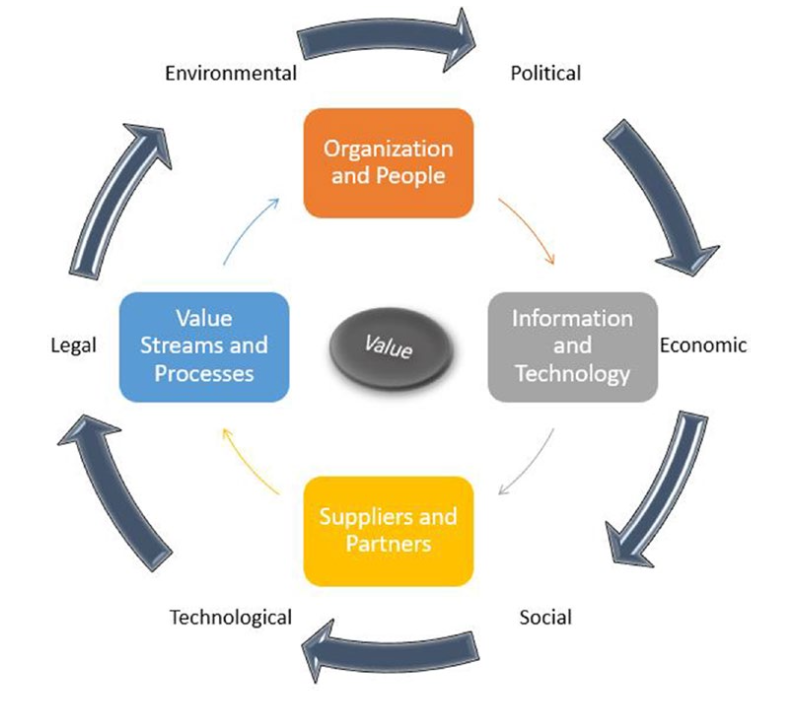
\includegraphics[width=0.5\linewidth]{images/image-01.png}
\end{center}
\end{frame}

\begin{frame}
	\frametitle{External Factors and the Four Dimensions}
	\begin{itemize}
		\item IT services don't operate in a vacuum.
		\item Rapid changes in the environment affect services.
		\item External factors influence service management.
		\item Four dimensions apply to every IT service.
		\item Categorization helps rejuvenate and balance service components.
	\end{itemize}
\end{frame}

\begin{frame}
	\frametitle{Organization and People}
	\begin{itemize}
		\item Services are run by people guided by organizations.
		\item Organization and people form the first dimension.
		\item Key aspects include:
		\begin{itemize}
			\item Organization structures
			\item Culture
			\item Roles and responsibilities
			\item Leadership
		\end{itemize}
		\item Human resources is a vast and continuously developing field.
	\end{itemize}
\end{frame}

\begin{frame}
	\frametitle{Bird’s-Eye View of Organization Structures}
	\begin{itemize}
		\item Organizations vary in size and structure.
		\item Structures are chosen based on the organization's needs.
		\item Current trend favors horizontal structures.
		\item Large organizations often require vertical structures.
		\item Agile organizations tend to have flat structures.
		\item Vertical structures are process-driven.
		\item Structure impacts service delivery effectiveness.
	\end{itemize}
\end{frame}

\begin{frame}
	\frametitle{Culture in Organizations}
	\begin{itemize}
		\item Culture is crucial for organization effectiveness.
		\item It's more impactful than the structure alone.
		\item Culture is about the organization's psychology.
		\item Important cultural questions:
		\begin{itemize}
			\item Ethics and transparency
			\item Respect for employee aspirations
			\item Promotion of open communication
		\end{itemize}
		\item Culture affects employee satisfaction and value creation.
	\end{itemize}
\end{frame}

\begin{frame}
	\frametitle{People Roles and Responsibilities}
	\begin{itemize}
		\item People are central to service delivery.
		\item Organizational structure and culture are foundations.
		\item Right people are critical for success.
		\item Leadership plays a key role in team selection.
		\item Roles and responsibilities must align with aspirations.
		\item Flat organizations have broader roles.
		\item Vertical organizations have more specialized roles.
	\end{itemize}
\end{frame}

\begin{frame}
	\frametitle{Leadership and Value}
	\begin{itemize}
		\item Leadership is crucial in guiding teams.
		\item Leaders must understand the organization's true north.
		\item Different leadership styles can be effective.
		\item All efforts should lead to value creation.
		\item Value is the ultimate goal of service management.
	\end{itemize}
\end{frame}

\begin{frame}
	\frametitle{Information and Technology in Service Management}
	\begin{itemize}
		\item Information and technology are distinct but connected.
		\item Information refers to knowledge and data.
		\item Technology involves tools like servers, software, etc.
		\item Two main areas of focus:
		\begin{itemize}
			\item IT for actual services
			\item IT for service management
		\end{itemize}
		\item Both areas are critical for service effectiveness.
	\end{itemize}
\end{frame}

\begin{frame}
	\frametitle{IT for Actual Services and Service Management}
	\begin{itemize}
		\item IT for services involves technology used by customers.
		\item IT for service management supports service delivery.
		\item Example: Netflix's servers and content delivery.
		\item Service management systems aid in seamless service.
		\item Buffering issues in streaming are managed by service IT.
		\item Service management systems aim to enhance user experience.
	\end{itemize}
\end{frame}

\begin{frame}
	\frametitle{Considerations for Information Management}
	\begin{itemize}
		\item Information management must be secure and compliant.
		\item Identify necessary information for service delivery.
		\item Ensure encryption and protection of stored information.
		\item Manage information updates and changes securely.
		\item Regulatory compliance (e.g., GDPR) is crucial.
		\item Information must be accessible yet protected.
	\end{itemize}
\end{frame}

\begin{frame}
	\frametitle{Partners and Suppliers}
	\begin{itemize}
		\item Third dimension of service management
		\item Focuses on external dependencies
		\item Cooperation and collaboration are norms
		\item Companies need partners for raw materials, network, or HR
		\item Aim for consistent and continuous relationships
		\item Deals should be win-win
		\item ITIL identifies this as a key dimension in service management
	\end{itemize}
\end{frame}

\begin{frame}
	\frametitle{Differentiating Partners and Suppliers}
	\begin{itemize}
		\item Supplier roles and responsibilities are clear
		\item Partnership is more than a customer-supplier relationship
		\item Partners have privileges, trust, and influence in decision-making
		\item Examples: Microsoft partnership for software licenses
		\item Suppliers: Transaction-based with no long-term commitment
		\item Example: Stationery mart versus Amazon Prime membership
	\end{itemize}
\end{frame}

\begin{frame}
	\frametitle{Partners vs. Suppliers}
	\begin{itemize}
		\item Partners: Built on trust, long-term commitment
		\item Suppliers: Transaction-based, contract-driven
		\item Partners share goals, culture, business environment
		\item Suppliers provide goods and services without ongoing relationship
		\item Example: Amazon Prime as a partner versus generic suppliers
	\end{itemize}
\end{frame}

\begin{frame}
	\frametitle{Organization Strategy for Partners and Suppliers}
	\begin{itemize}
		\item Decision to buy or build versus outsourcing
		\item Cost considerations and efficiency
		\item Talent availability and outsourcing
		\item Industry trends and risk management
		\item Legal and regulatory requirements impact decisions
	\end{itemize}
\end{frame}

\begin{frame}
	\frametitle{Introducing Service Integration and Management (SIAM)}
	\begin{itemize}
		\item Framework for managing partners and suppliers
		\item Acts as an interface between customer and partners
		\item Manages strategic, tactical, and transaction activities
		\item Can be third-party or internal division
		\item Ensures effective management of all partners and suppliers
	\end{itemize}
\end{frame}

\begin{frame}
	\frametitle{Value Streams and Processes}
	\begin{itemize}
		\item Value streams: Coordinated steps to co-create value
		\item Difference between process and value stream
		\item Process: Transforms inputs into outputs
		\item Value stream: Focuses on eliminating waste and improving productivity
		\item Example: Barber’s service value stream
	\end{itemize}
\end{frame}

\begin{frame}
	\frametitle{Deciphering Value Streams}
	\begin{itemize}
		\item Operating model for value creation
		\item ITIL service value chain
		\item Value streams: Patterns for delivering value
		\item Identify and reduce waste
		\item Example: Optimizing barber's service
	\end{itemize}
\end{frame}

\begin{frame}{Illustration of a service value stream}
	 \frametitle{ Illustration of a service value stream}
\begin{center}
	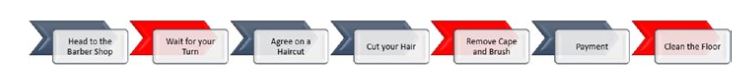
\includegraphics[width=0.8\linewidth]{images/image-02.png}
\end{center}
\end{frame}

\begin{frame}
	\frametitle{Simplifying Processes}
	\begin{itemize}
		\item Process: Set of interrelated activities
		\item Transforms inputs into outputs
		\item Example: Recipe for making an egg omelet
		\item Processes define action sequences and dependencies
	\end{itemize}
\end{frame}

\begin{frame}
	\frametitle{PESTLE Analysis}
	\begin{itemize}
		\item External factors influencing services and products
		\item Political, Economic, Social, Technological, Legal, Environmental
		\item Examples: Covid-19 impact, economic downturns, technological advancements
	\end{itemize}
\end{frame}

\begin{frame}
	\frametitle{Political Factors}
	\begin{itemize}
		\item Impact of political actions and legislation
		\item Example: Covid-19 lockdown and remote work adaptations
	\end{itemize}
\end{frame}

\begin{frame}
	\frametitle{Economic Factors}
	\begin{itemize}
		\item Budgeting and cost management
		\item Example: Cost cuts due to economic downturns
	\end{itemize}
\end{frame}

\begin{frame}
	\frametitle{Social Factors}
	\begin{itemize}
		\item Changes in societal needs and wants
		\item Example: Nokia’s failure to adapt to touch screens
	\end{itemize}
\end{frame}

\begin{frame}
	\frametitle{Technological Factors}
	\begin{itemize}
		\item Importance of technological upgrades
		\item Example: Blockbuster’s failure to adopt streaming technology
	\end{itemize}
\end{frame}

\begin{frame}
	\frametitle{Legal Factors}
	\begin{itemize}
		\item Compliance with laws and regulations
		\item Example: GDPR impact on digital channels
	\end{itemize}
\end{frame}

\begin{frame}
	\frametitle{Environmental Factors}
	\begin{itemize}
		\item Influence of environmental changes
		\item Example: Demand for organic products and services
	\end{itemize}
\end{frame}

\begin{frame}
	\frametitle{Quiz Question}
	Which of the options accurately reflects the difference between a partner and a supplier?
	
	\begin{enumerate}[A.]
		\item Clear separation of roles
		\item Partners maintain knowledge bases
		\item Suppliers are managed by partners
		\item Partners are managed by suppliers
	\end{enumerate}
\end{frame}


\end{document}
